\chapter{Background}

\label{Background}

%\lhead{Chapter 2. \emph{Background}}

\section{Plagiarism Detection}

Though our primary aim is to provide insightful analysis of the students' code 
submissions and not to detect plagiarism, a lot of our research took 
place in the realm of plagiarism detection. In detecting plagiarism, programs are attempting
to output a binary result of ``plagiarism detected'' or ``no plagiarism detected''.
To accomplish this, however, the programs must first build a representation of 
how similar the code is, and then flag code which is similar above a certain threshold.
It is now clear why we should leverage this research -- to reliably detect plagiarism,
we must first reliably judge similarity.

Code similarity detection techniques have been divided up into a number of subclasses:
text, token, source tree, PDG (Program Dependency Graph) based\cite{CloneDetection}.

Textual analysis is a popular area of research in plagiarism
detection. Analysis of this type is the most na\"{\i}ve; there is no leveraging
of our knowledge of the files we are comparing. Generally these algorithms
will compare two pieces of code by considering them both as a sequence of
strings (often using a line per string), matching the number of identical
strings or finding the longest sequence of matching strings. 
Optimisations or improvements of this approach will remove comments and whitespace
and apply normalisation on the source code. This normalisation involves replacing
certain types of elements with a uniform replacement, as described in 
\cref{tab:normalise}. An example of these optimisations can be see in 
\cref{code:optimisedText}. The exact similarity value calculated depends -- as
with most general approaches in this area -- on the specific algorithm used.
For example Ducasse et. al\cite{DucasseText} apply all previously mentioned optimisations,
and iterate over each line, performing a string comparison algorithm to recognise
the longest subsequence matches. We can see how removing the comments,
whitespace and other uninteresting language constructs would improve string
matching, as these sections don't change the semantics of code, yet could cause
misses in the matching algorithm if people used different comments etc. in
their solutions, as is expected, and they were retained.

\begin{figure}[h!]
\label{tab:normalise}
\begin{tabular}{| l | l | l |}
\hline 
\textbf{Language element} & \textbf{Example} & \textbf{Replacement} \\
\hline \hline
Literal string & ``Abort'' & ``...'' \\
\hline
Literal character & `y' & `.' \\
\hline
Literal integer & 42 & 1 \\
\hline
Literal decimal & 0.314159 & 1.0 \\
\hline
Identifier & counter & p \\
\hline
Basic numerical type & int, short, long, double & num \\
\hline
Function name & main & foo() \\
\hline \hline
\end{tabular}
\caption{Normalization table as used in text based approaches\cite{DucasseText}}
\end{figure}
\begin{figure}[h!]
\begin{tabular}{l l l}
\textbf{Original Code} & \textbf{After Normalising} & \textbf{After Filtering} \\
\texttt{include stdio.h} & \texttt{include lib} & \\
\texttt{static int stat = 0;} & \texttt{mod num var = 1;} & \texttt{modnumvar=0;}\\
\texttt{int main(argc, argv)} & \texttt{num foo(p,p)} & \texttt{numfoo(p,p)}\\
\texttt{  int argc;} & \texttt{  num p;} & \texttt{nump;}\\
\texttt{  char **argv;} & \texttt{  ptr p;} & \texttt{ptrp;}\\
\texttt{\{} & \texttt{\{} & \texttt{opp,opp;}\\
\texttt{  /*skip program name*/} & \texttt{  /*skip program name*/} & \texttt{if(pop1)}\\
\texttt{  ++argv, --argc;} & \texttt{  opp, opp;} & \\
\texttt{  if(argc > 0) \{} & \texttt{  if(p op 1)\{} & \\
\end{tabular}
\caption{Text-based optimisations; Adapted from\citep[p.~49]{CloneDetection}}
\label{code:optimisedText}
\end{figure}

Token based approaches take on a more intelligent approach to similarity analysis
than textual analysis, however the fundamental idea behind token analysis is similar.
Initially, the source code is lexed, or otherwise transformed, into a sequence of tokens.
From here we can perform analysis on the sequences to determine similarity, as described
below.

A number of different algorithms have been developed for this purpose.
MOSS is a popular tool used throughout academia for detecting plagiarism
in code, which accepts a large number of input source code files and uses 
its own method to check for plagiarism. The technique used is known as 
``winnowing''~\cite{winnowing}. This process takes ideas from earlier detection
techniques, such as \emph{k-grams}, and applies their own algorithms to indicate
code duplication. The \emph{k-gram} approach involves splitting the source code up into
strings of length $k$, ($k$ is defined by the user and is implementation specific).
The winnowing algorithm works by hashing the \emph{k-grams} and moving through 
\emph{windows}, $w$ consecutive \emph{k-gram} hashes.
The winnowing step is the defined as: 
\begin{quote}In each window select the minimum hash value.
If there is more than one hash with the minimum value, select the rightmost
occurence. Now save all selected hashes as the fingerprints of the document.
\cite{winnowing}
\end{quote}

This process is undertaken after refactoring the code so that whitespace
has minimal effect and, if possible, variable renaming to normalised names.
The resulting fingerprints are then compared with the fingerprints of another
code base, with more hits indicating a larger likelihood of plagiarism.

\begin{figure}[h!]
\begin{minipage}[b]{0.45\linewidth}
\begin{lstlisting}[language=Java]
int len = 5;
int[][][] myArr = new int[len][len][len];
for(int x = 0; x < len; x++) {
	for(int y = 0; y < len; y++) {
		for(int z = 0; z < len; z++) {
			myArr[x][y][z] = x+y+z;
		}
	}
}
\end{lstlisting}
\caption{A simple for-loop}
\label{fig:xyzForLoopBG}
\end{minipage}
\hspace{0.5cm}
\begin{minipage}[b]{0.45\linewidth}
\begin{lstlisting}[language=Java]
int size = 5;
int[][][] nums = new int[size][size][size];
for(int i = 0; i < size; i++) {
	for(int j = 0; j < size; j++) {
		for(int k = 0; k < size; k++) {
			nums[i][j][k] = i+j+k;
		}
	}
}
\end{lstlisting}
\caption{A semantically identical for-loop to \cref{fig:xyzForLoopBG}}
\label{fig:ijkForLoopBG}
\end{minipage}
\end{figure}

We can see how this could be applicable for the uses of code similarity -- 
where code is written in a similar manner, more fingerprints would match,
giving us a high similarity score. Though this process works for plagiarism detection
where it is expected that code is simply lifted from one student's work to
another's, concerns can be raised as to how applicable this technique will work
when the code is similarly written, but not a direct copy. For example, when 
students are applying the same ideas to write their code, but not actually
copying each other, we would want to see a high similarity score. It is possible
that this may not result in a high score through winnowing as the \emph{string
similarity} of two pieces of code could be low, whilst they actually perform
the same function in the same manner. \cref{fig:xyzForLoopBG} and
\cref{fig:ijkForLoopBG} illustrate this concern -- there are no matching
textual comparisons in the code snippet, except for the traditional java
keywords and structures. Choosing a window which is small enough for
these two functions to match, e.g. by matching with the string 
``++)\{for(int'', would essentially allow most for-loops to match throughout
the source files; anything larger and the two loops wouldn't match at all.

Other token based methods are similar in form, but perform
more complex preprocessing on the code to gain more insight into code similarity.
One example converts code into specific tokens, such as \texttt{BEGIN\_CLASS}, \texttt{VAR\_DEF}
etc., as shown in \cref{fig:JPlagTokenCreation}. These token arrays are 
compared between files with ``Greedy String Tiling''\cite{GreedyStringTiling}.
The largest matching tiles are selected from the tokenised arrays and a similarity
calculated between the files using their similarity function:
\[sim(A,B) = 2 \cdot
coverage(tiles)/(|A| + |B|)\] where \[coverage(tiles) =
\sum\nolimits_{match(a,b,length) \in tiles}length\]
\cite{JPlag}

\begin{figure}[H]
\begin{tabular}{l l}
\textbf{Java source code} & \textbf{Generated tokens} \\
\lstinline[language=Java]!public class Count! & BEGIN\_CLASS \\
\lstinline[language=Java]!    public static void main(String[] args)! & VAR\_DEF, BEGIN\_METHOD \\
\lstinline[language=Java]!            throws java.io.IOException {! \\
\lstinline[language=Java]!        int count = 0;! & VAR\_DEF, ASSIGN \\
\lstinline[language=Java]!        while (System.in.read() != -1)! & APPLY, BEGIN\_WHILE \\
\lstinline[language=Java]!            count++;! & ASSIGN, END\_WHILE \\
\lstinline[language=Java]!        System.out.println(count+" chars.");! & APPLY \\
\lstinline[language=Java]!    }! & END\_METHOD \\
\lstinline[language=Java]!}! & END\_CLASS \\
\end{tabular}
\caption{Taken from \citep[p.~1020]{JPlag}}
\label{fig:JPlagTokenCreation}
\end{figure}


PDG analysis is based on the idea of abstracting your programs, and generating
graphs based on the flow of code, in particular the branching of conditionals
and access to data\cite{PDGOptimisation}. The structure of these graphs
is generally invariant under plagiarism, as it is robust to changes in line
orders, additional comments and whitespace\cite{GPLAG}. As a result, the technique is well
suited to plagiarism and therefore similarity detection. Numerous studies have been based
on the PDG approach to plagiarism detection\cite{GPLAG} \cite{OtherPDG}, giving
interesting results into its applicability.

There is a small amount of research which analyses the parse trees
of the code directly. Though sparse, the work in this area is interesting
to examine. Early work \cite{Belkhouche} involves a number of steps to get
a similarity score. Initially, the AST of the code is generated and transformed
into a structure chart. This is essentially a modified form of the AST;
the structure chart consists of two parts the tree, and the data dictionary
containing the variables and data types used in the code\cite{Belkhouche}. This structure
chart is partitioned into regions based upon their type (sequential, repetition
and selection), with the partitioning applied recursively until the partitions
have at least one statement. The partitioning of two pieces of code, defined in
\cref{code:belkhouche1} and \cref{code:belkhouche2}, are shown in
\cref{fig:belkhoucheRegions1} and \cref{fig:belkhoucheRegions2}. These regions
now make up an abstract region tree, which undergo abstract comparison. For
each level of the region tree, compare the nodes in the tree, scoring a similarity
based on the number of matching nodes. Regions with a high enough similarity,
for example 50\%, are used in the next step. For the remaining regions, the code
is scrutinised more closely with a novel \emph{micro comparison} step. Each
leaf node left in the graph is now a statement such as \texttt{foo(x)} or
\texttt{y = bar}; we can create trees from each of these leaf nodes
looking at the shape and tokens of evaluation subtrees to look for similarity. 
Each subtree can be compared on shape and the value of its nodes, the shape
giving information about the semantics of the statement, whilst the tokens
indicate similar syntax.
The data dictionary of the two trees are finally compared, comparing the number
of variables of each type, and also the (variable type, variable id) pairs.
Each step contributes to the similarity scoring of the two, and finally an output
of plagiarism suspicion is given.

\begin{figure}[p]
\begin{lstlisting}[language=C, numbers=left]
big = 0;
PandR(x);
PandR(y);
PandR(z);
if(x > y) {
	if(x > z) {
		big = x;
	} else {
		big = z;
	}
} else {
	if(y > z) {
		big = y;
	} else {
		big = z;
	}
}
cnt = 0;
sqr = 0;
if(big > 0) {
	if(cnt < big) {
		sqr = sqr + big;
		cnt = cnt + 1;
	}
	cnt = 0;
}
return sqr;
\end{lstlisting}
\caption{Example code used in \cref{fig:belkhoucheRegions1}}
\label{code:belkhouche1}

\begin{lstlisting}[firstnumber=18, language=C, numbers=left]
cnt = 0;
sqr = 0;
sqr = 0;
\end{lstlisting}

\begin{lstlisting}[firstnumber=27, language=C, numbers=left]
}
sqr = sqr;
return sqr;
\end{lstlisting}
\caption{Simple modifications of \cref{code:belkhouche1} as outlined in
\cref{fig:belkhoucheRegions2}}
\label{code:belkhouche2}
\end{figure}


\begin{figure}[p]
	\centering
		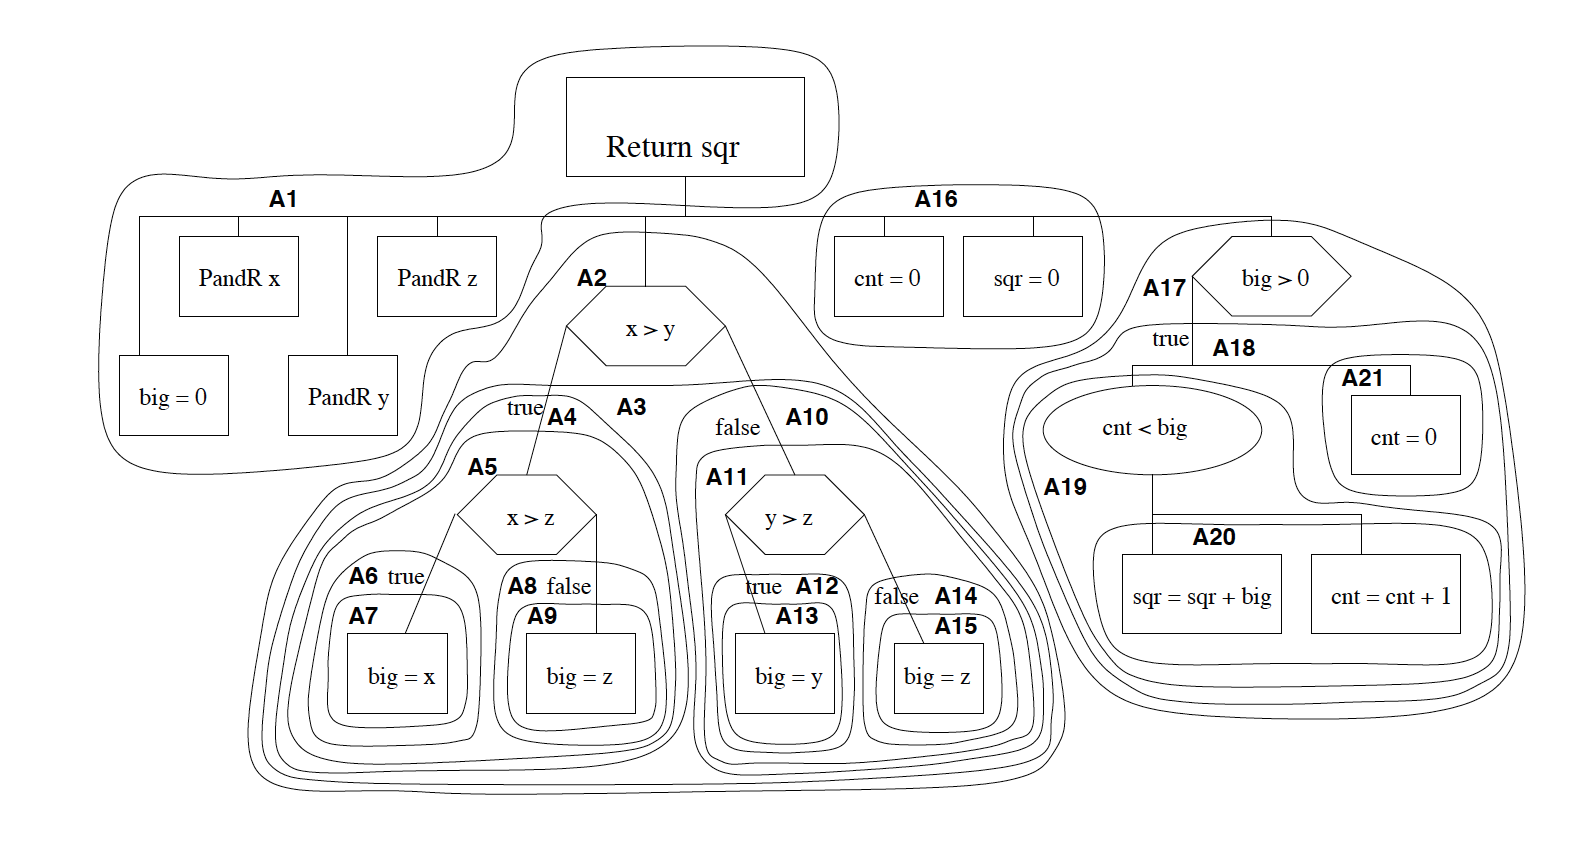
\includegraphics[width=\textwidth]{Figures/Belkhouche1}
	\caption{Regions specified for the code in \cref{code:belkhouche1} with Belkhouche et. al's method~\cite{Belkhouche}}
	\label{fig:belkhoucheRegions1}
	
	\centering
		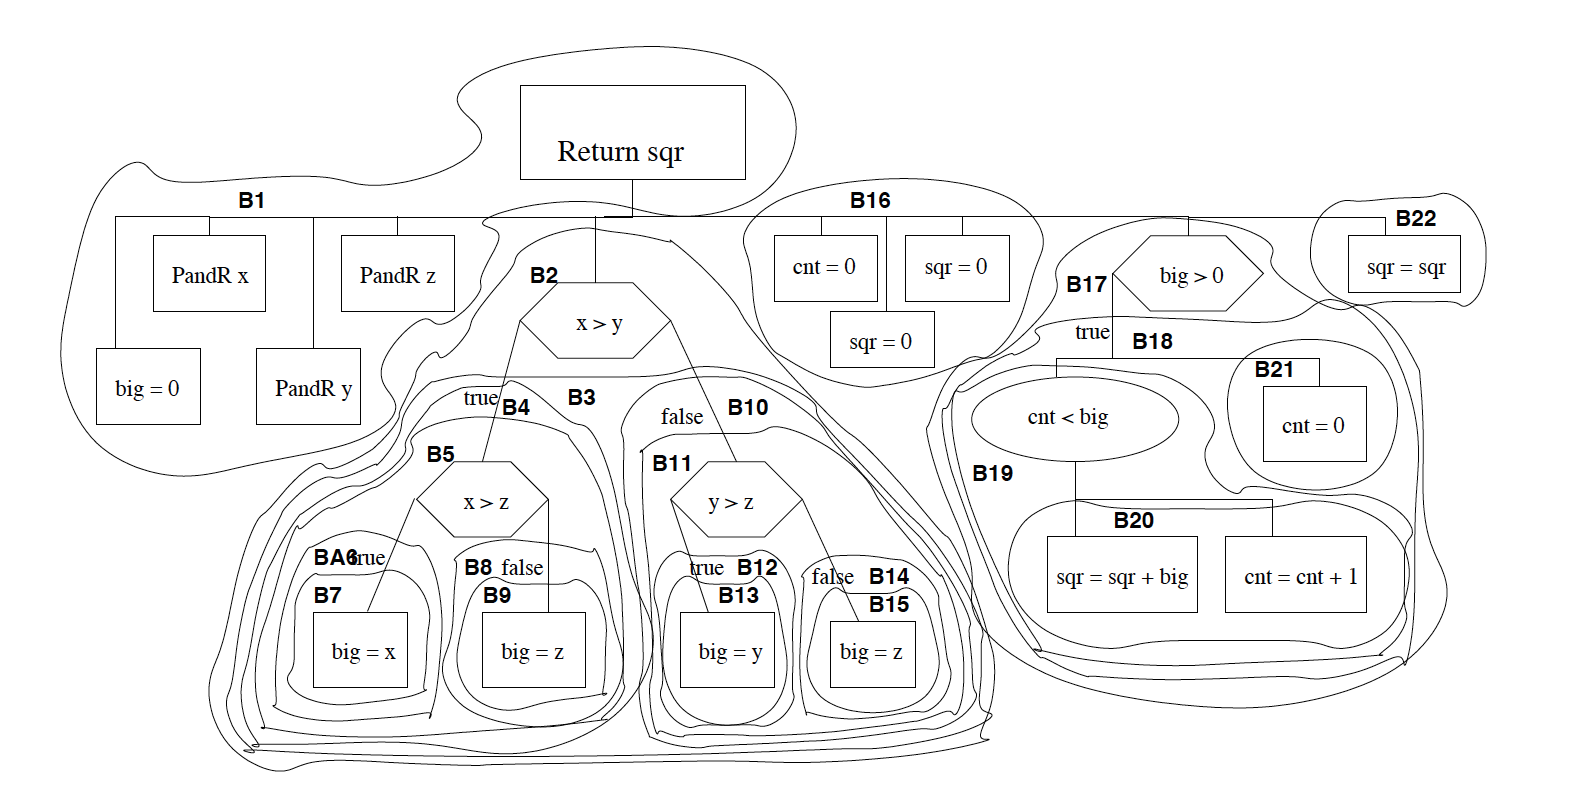
\includegraphics[width=\textwidth]{Figures/Belkhouche2}
	\caption{Regions specified for the code in \cref{code:belkhouche2} with Belkhouche et. al's method~\cite{Belkhouche}}
	\label{fig:belkhoucheRegions2}

\end{figure}

Building on the work of \cite{Belkhouche}
we came across a recently published algorithm based on a parse tree kernel function
\cite{ParseTreeKernel}. The parse tree kernel function has its roots
in Natural Language Processing, in particular ``Convolution Kernels'' for natural
language\cite{NLPKernel}. A kernel function between two data sets is an ``evaluation
of the dot product between pairs of examples''\cite{NLPKernel}. It is possible
to apply a kernel function to a many-dimensional space and efficiently calculate
the result of some function between the two data sets. The explanation of the
kernel functions is a rather confusing justification, however the intuition
becomes clear when described step by step.

The initial convolution kernel function aims at detecting similarity in the
natural language space. As such, it defines rules which do not seem
appropriate for code analysis, however the fundamental ideas are still applicable,
hence the foundation of the code analysis function in NLP.

The kernel function between two trees is defined as:

\begin{equation}
K(T\textsubscript{1}, T\textsubscript{2}) = \mathbf{h}(T\textsubscript{1})
\cdot \mathbf{h}(T\textsubscript{2})
\end{equation}
To calculate this, we define the set of nodes in $T\textsubscript{1}$ and 
$T\textsubscript{2}$ as $N\textsubscript{1}$ and $N\textsubscript{2}$. We
also define an indicator function $I\textsubscript{i}(n)$ as 1 if the 
tree $i$ is rooted at node $n$, 0 otherwise. As described in \cite{NLPKernel}
we therefore get the following:

\begin{equation}
\textbf{h}(T\textsubscript{1}) \cdot \textbf{h}(T\textsubscript{2}) =
\sum_{i}{h\textsubscript{i}(T\textsubscript{1})h\textsubscript{i}(T\textsubscript{2})} =
\sum_{n\textsubscript{1}\in N\textsubscript{1}} \sum_{n\textsubscript{2} \in N\textsubscript{2}}
\sum_{i}{I\textsubscript{i}(n\textsubscript{1})I\textsubscript{i}(n\textsubscript{2})} =
\sum_{n\textsubscript{1}\in N\textsubscript{1}} \sum_{n\textsubscript{2} \in N\textsubscript{2}}
{C(n\textsubscript{1}, n\textsubscript{2})}
\end{equation}

If the productions (i.e. the type of the node and the type and order of its 
child nodes) at $n\textsubscript{1}$ and $n\textsubscript{2}$ are different
then:

\begin{equation}
C(n\textsubscript{1}, n\textsubscript{2}) = 0
\end{equation}

If the productions at $n\textsubscript{1}$ and $n\textsubscript{2}$ are the same,
and $n\textsubscript{1}$ and $n\textsubscript{2}$ are pre-terminals (nodes directly
above the terminal nodes) then:

\begin{equation}
C(n\textsubscript{1}, n\textsubscript{2}) = 1
\end{equation}

Else:

\begin{equation}
C(n\textsubscript{1}, n\textsubscript{2}) = \prod_{j=1}^{nc(n\textsubscript{1})}
{(1+C(ch(n\textsubscript{1}, j), ch(\textsubscript{2}, j)))}
\end{equation}

where $nc(n\textsubscript{1})$ is the number of children of $n\textsubscript{1}$.

For plagiarism detection of code, the parse tree kernel given above must be
modified majorly to deal with the problems that come from source code
\cite{ParseTreeKernel}. Some of the features of source code that make modifications
necessary include the size of the parse tree. Generally natural language parse
trees will be fairly small in size; by comparison the parse tree of a program can
grow much deeper, with nested loops, inner classes etc. It can be seen that the
depth of a large tree is an issue as when a root node, or a node near the root,
is modified, the change has a much bigger influence on the result than if
the change appeared further towards the leaves -- given that the parse tree 
kernel uses all subtrees of a tree\cite{ParseTreeKernel}. 

\begin{figure}[H]
	\centering
		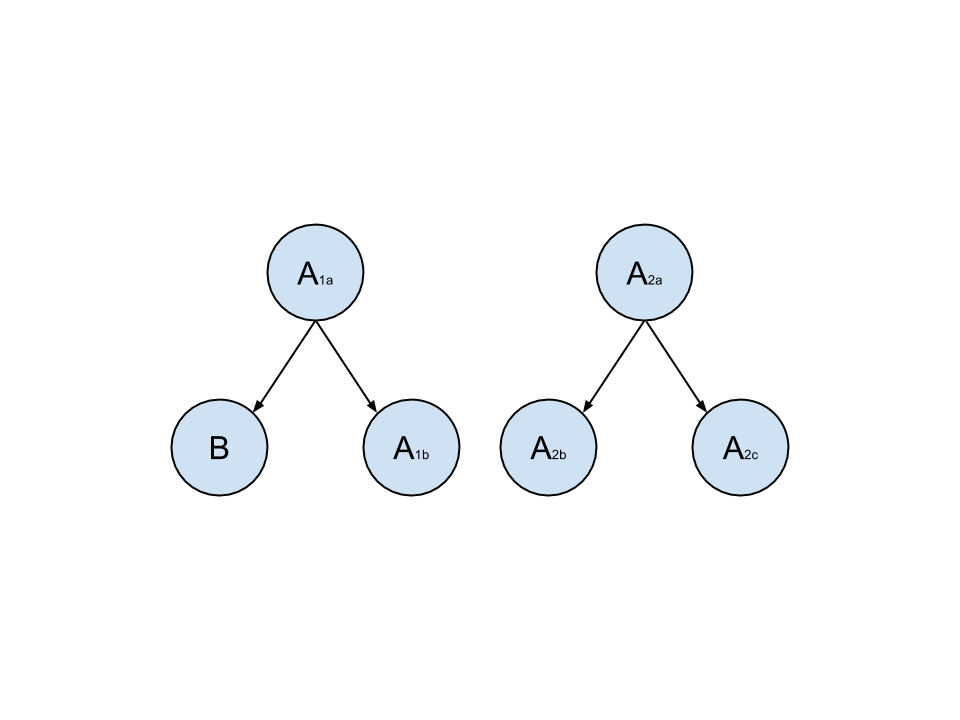
\includegraphics[width=\textwidth]{Figures/SimpleParseTree}
	\caption{An example parse tree we can apply the steps of the parse tree kernel
	algorithm to}
	\label{fig:SimpleParseTree}
\end{figure}

This concern is avoided with the introduction of a \emph{decay factor},
$\lambda$ defined as $0 < \lambda \le 1$. This factor is applied to each
level of the tree, reducing the weighting of each level exponentially.
As such, large subtrees have a much smaller weighting than they otherwise
would\cite{ParseTreeKernel}. Deep subtrees still have an effect with this factor
applied, and as such, there is another constant introduced, the \emph{threshold
depth}, $\Delta$. This value limits the function such that the max subtree depth
to be evaluated is $\Delta$. This completely removes the ``disproportionate influence
of near-root level changes''\cite{ParseTreeKernel}.

Applying the values, we modify the equations before to give the rules below.

If the productions at $n\textsubscript{1}$ and $n\textsubscript{2}$ are different
then:
\begin{equation}
C(n\textsubscript{1}, n\textsubscript{2}) = 0
\end{equation}

If both $n\textsubscript{1}$ and $n\textsubscript{2}$ are pre-terminals or the
current depth is $\Delta$ then:

\begin{equation}
C(n\textsubscript{1}, n\textsubscript{2}) = \lambda
\end{equation}

Else:

\begin{equation}
C(n\textsubscript{1}, n\textsubscript{2}) = \lambda\prod_{i}^{nc(n\textsubscript{1})}
{(1+C(ch(n\textsubscript{1}, j), ch(\textsubscript{2}, j)))}
\end{equation}
\cite{ParseTreeKernel}

Taking note of the definition of productions, we see another error with this
approach to source code -- the number of children of a node of a certain type
are unlikely to be the same even when code is similar. For example, if a function
is split into two, but performs the exact same function, the children of a
\emph{class definition} would change. Further to this, the algorithm currently
only checks the nodes in order, i.e. the $i$th child of $n\textsubscript{1}$ is
compared with the $i$th child of $n\textsubscript{2}$ only. In source code, we
can usually change the order of statements without affecting the the semantics
of the program. These observations result in another change to the equation.

If $n\textsubscript{1}$ and $n\textsubscript{2}$ are different (this is understood
to mean, if the types of the node are different, e.g. a \emph{method declaration}
node and a \emph{variable assignment} node)
then:
\begin{equation}\label{eq:parseTreeKernelBase1}
C(n\textsubscript{1}, n\textsubscript{2}) = 0
\end{equation}

If both $n\textsubscript{1}$ and $n\textsubscript{2}$ are terminals or the
current depth is $\Delta$ then:

\begin{equation}\label{eq:parseTreeKernelBase2}
C(n\textsubscript{1}, n\textsubscript{2}) = \lambda
\end{equation}

Else, we have two options:

\begin{enumerate}
\item Maximum node value, MNV:
\begin{equation}\label{eq:parseTreeKernelRecurse}
C(n\textsubscript{1}, n\textsubscript{2}) = \lambda\prod_{i}^{nc(n\textsubscript{1})}
{(1+\max_{ch \in ch \textsubscript{n\textsubscript{2}}}{C(ch\textsubscript{i}
(n\textsubscript{1}), ch))}}
\end{equation}

\item Mean value, MV:
\begin{equation}
C(n\textsubscript{1}, n\textsubscript{2}) = \lambda\prod_{i}^{nc(n\textsubscript{1})}
{(1+\mathrm{E}_{ch \in ch \textsubscript{n\textsubscript{2}}}{[C(ch\textsubscript{i}
(n\textsubscript{1}), ch)])}}
\end{equation}
\end{enumerate}
\label{secondImprovementParseTreeKernel}

The authors have opted for the MNV variant of the recursive case, justifying
as their aim is to detect plagiarism, and therefore want the highest similarity.
For source code similarity, there is an arugment to take either approach; 
using the MV should give an average of how similar each node is
against every node in the tree, which does seem a wanted attribute. There is,
however also a case in using the MNV -- take the example of a node
of \emph{class definition} with a large number of child nodes. If this
node's children are all-but-one of the type \emph{field declaration}, with one
node being a \emph{method declaration}, passing in a \emph{class definition} node
with one child -- an identical \emph{method declaration} to the first tree -- we'd
want to recognise that this node had a high similarity. We could also argue that
if the node doesn't match with the many other child nodes, then it would be
misrepresentative to indicate a high similarity when there are so many unmatched
nodes. This uncertainty stems from, as previously discussed, the lack of concensus
in code similarity.

Regardless of the final measure taken, the final output of $k(T\textsubscript{1},
T\textsubscript{2})$ is an unnormalised value. The value returned varies 
based on the size of the trees e.g. two large, vaguely similar trees 
could return a much larger value than two tiny trees that are identical. As
such a normalised step is defined such that:

\begin{equation}\label{eq:normalise}
N(s,s') = \frac{k(s, s')}{\sqrt{k(s, s) \cdot k(s', s')}}
\end{equation}

This ensures that the similarity between $s$ and $s'$, is bounded such that 
$0 \le N(s, s') \le 1$.

A worked example can be seen with \cref{fig:SimpleParseTree}. To calculate
$K(T\textsubscript{1}, T\textsubscript{2})$, we need to find the sum of
calls to C for every combination of nodes in the trees.

\begin{equation}
C(A\textsubscript{1a}, A\textsubscript{2a}) = 
\lambda(1+\max_{ch\in ch\textsubscript{A\textsubscript{2a}}}{C(B\textsubscript{1}, ch)})
(1+\max_{ch\in ch\textsubscript{A\textsubscript{2a}}}{C(A\textsubscript{1b}, ch)})
\end{equation}

We know that $C(B\textsubscript{1}, n\textsubscript{2}) = 0$ as the second tree
doesn't contain any \emph{B} nodes and the rules in \cref{eq:parseTreeKernelBase1}. 
The second recursive call to C 
($C(A\textsubscript{1b}, ch)$), will return $\lambda$ for both child nodes as
they are the same type via \cref{eq:parseTreeKernelBase2}. Therefore 
\begin{equation}
C(A\textsubscript{1a}, A\textsubscript{2a}) = \lambda(1+\lambda)(1+0)
= \lambda(1+\lambda)
\end{equation}

as the leaf nodes have no children, the product for the case of 
$C(A\textsubscript{1a}, A\textsubscript{2b})$ and $C(A\textsubscript{1a}, A\textsubscript{2c})$ 
simply returns $\lambda$ both times.

As stated, comparing $B\textsubscript{1}$ with each node in $T\textsubscript{2}$ will
return 0.

Finally, the node $A\textsubscript{1b}$ will be compared with each node in turn.
When comparing it with the root node $A\textsubscript{2a}$, we see that 
$nc(A\textsubscript{1b}) == 0$ therefore no values come out of the product and
$\lambda$ is returned. By \cref{eq:parseTreeKernelBase2}, when comparing the
node with both $A\textsubscript{2b}$ and $A\textsubscript{2c}$, we get $\lambda$
both times.

As the similarity requires the sum of these calls to C:

\begin{equation}
k(T\textsubscript{1}, T\textsubscript{2}) = \lambda(1+\lambda) + 5\lambda
\end{equation}

assuming $\Delta > 1$.

The algorithm discussed uses two values, \emph{threshold depth} and 
\emph{decay factor}, to calculate the similarity. The paper claims in their
experiments that they were heuristically set to 3 and 0.3 respectively.
Unfortunately no insight is given in \cite{ParseTreeKernel} as to how these
values are calculated, so any implementation would have to experiment with
different values for these, to see which gives the best performance.
This does, however, leave any implementation in danger of overtraining
when trying to choose the best values. Despite this drawback, the algorithm does
provide a unique take on the parse tree approach to similarity analysis. According
to the results \cite{ParseTreeKernel}, it preforms better than the more established
programs (JPlag etc.) for certain cases of code plagiarism. This is a promising
direction to take similarity analysis.

Of the techniques discussed, the parse tree approach is an area with only a small
amount of research. There are many well established applications using other
similarity measure, such as JPlag\cite{JPlag} and MOSS\cite{winnowing}, 
but none that focus on parsing the code with the aim of
analysing the tree. It would be interesting to look at the possibilities this
technique provides us, with potentially very rich information accessible to
lab coordinators from a tool based around the parse tree kernel algorithm.

\label{sec:parseTreeKernel}

\section{Parse Tree Retrieval Methods}

As we wish to look more at a parse tree approach to similarity analysis, we must
first look at how we are able to access the parse tree. Our current data sets of
student code is based in Haskell, Java, C and C++; the Haskell code base is rather
small and basic however as students initially learn this language as an introduction
to programming, therefore would likely give uninteresting results. The remaining
languages have all been studied extensively in plagiarism detection, we know the
structures in these languages are compatible with the algorithms put forward,
which is vital. Indeed, the main pieces of research into parse tree analysis
are based around C \cite{Belkhouche} and Java \cite{ParseTreeKernel}.

Other research has generally taken the route of using a lexer/parser generator,
such as flex\footnote{http://flex.sourceforge.net/} and 
bison\footnote{http://www.gnu.org/software/bison/} to generate their parse trees
for analysis. Whilst this is a perfectly valid approach, we felt it would be
ideal if we could plug directly in to a compiler used on the course. This
would ensure we don't need to concern ourselves with creating a grammar for a
language, as this is built in to the compiler. Instead, we would be able to
take the data structure from an intermediate stage of compilation and perform
analysis directly on it.

Our initial approach took us to the GCC compiler -- there is a very large
Operating Systems coursework and it would have been exciting to see what insights
we could gain around it. We found a great plugin 
framework\footnote{https://gcc.gnu.org/onlinedocs/gccint/Plugins.html}, which
allows developers to add features to GCC to be performed during compilation. The
plugin framework is so beneficial as it prevents users relying on extending
a particular version of the compiler, and being forced to update their features
as the compiler updates with incompatible changes. The compiler generates an
AST in a language specific format, however from here, transforms code into a
Generic/GIMPLE format, as demonstrated in \cref{fig:GCCFlow}. This format is
language independent and so our algorithm could be applied to any language
which has a GNU compiler.

\begin{figure}[H]
	\centering
		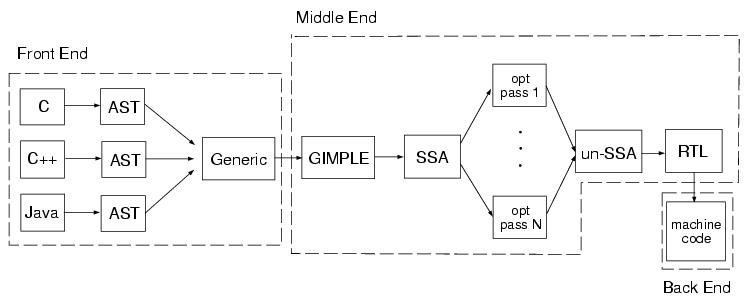
\includegraphics[width=\textwidth]{Figures/GCCFlow}\footnotemark{}
	\caption{The GCC compilation process}
	\label{fig:GCCFlow}
	
\end{figure}

Unfortunately, the GCC plugin framework had a major drawback -- when compiling
\footnotetext{http://en.wikibooks.org/wiki/File:GCC.JPG}
the code, we had full access to manipulate the parse tree, however there was
no way to store the tree in a format that allowed it to be rebuilt 
programmatically. A raw dump of the tree could be made, but no API was 
provided to parse this tree back into C. This was an issue as, with the complex
building process of the C coursework, it would be computationally infeasible
to parse and compile all courseworks together.

This led us to examine Eclipse, and its plugin framework.
The Eclipse IDE is a development environment for the Java programming language;
It provides tools for Java developers to write compile and debug their applications.
Further to this, it also provides a feature rich environment in which developers
can create additional plugins to add functionality to the base Eclipse distribution.

With access to this plugin framework, Eclipse exposes some of its internal APIs
and allows developers to be able to manipulate Java in complex ways. The key feature
of this, as it relates to us, is the ability to plug in to the Java compiler of Eclipse
and manipulate the Parse trees as we wish. This easy access to a parse tree in a
feature rich environment such as Eclipse was our main motivation behind the approach
to our primary application. Utilising the plugin environment, we could examine the
source code as it is parsed, and perform our comparison, all within the standard
compilation, with no external tools needed.

\section{Data Analysis -- Clustering}

With a huge array (NxN) of scores, it is infeasible to manually search through
these scores and pick out interesting trends. This led us to look for a data
analysis package that could provide a rich interface and is easy to use. There
are a number of data visualisation tools available as Java libraries that would
have been ideal to use. Prefuse\footnote{http://prefuse.org/} was a possibility, a free
to use, open source library. It provides support for visualisation of assorted
graphs, trees and tables, using its own SQL-like expression language to input
data. This library, however, is sparsely updated (the last commit being 10
months ago) and the documentation is lacking. As an example the `Graphs and
Trees' page of the manual informs us that the page is `Under Construction!
Coming soon'; the page was last updated in 2007.

Few other Java visualisation options were found, and so we looked for other
data visualisation packages. Orange\footnote{http://orange.biolab.si/} is a cross platform data
visualisation tool developed in python. It is an interesting package, having
a CLI to perform custom analyses, but also an easy to use GUI. The GUI uses
a widget toolkit to allow for easy data processing -- many types of nodes
are provided by the program, after selecting some of these, for example `Distance
File' and `Distance Map', they appear in the main application window. From here,
users can select the external inputs to the nodes (e.g. from files), and wire
together relevant components, configuring the output of one widget to be the
input to another. For example, in \cref{fig:orangeUI} we can see a distance file
-- a file which stores a triangular matrix of distances ($d>0$) between given labels --
is taken from external input. The Distance File node parses this, and can output
a matrix of distances, which are wired in to the Distance Map and Hierarchical Clustering
nodes. These nodes take an input of distances, with the Distance Map displaying a heatmap
of the input. The Hierarchical Clustering widget provides great utility, in that
it reads in our data matrix and performs a clustering of the data, based on
complete linkage. The complete linkage clustering algorithm works by assigning
all nodes to their own cluster. 
\begin{figure}[H]
	\centering
		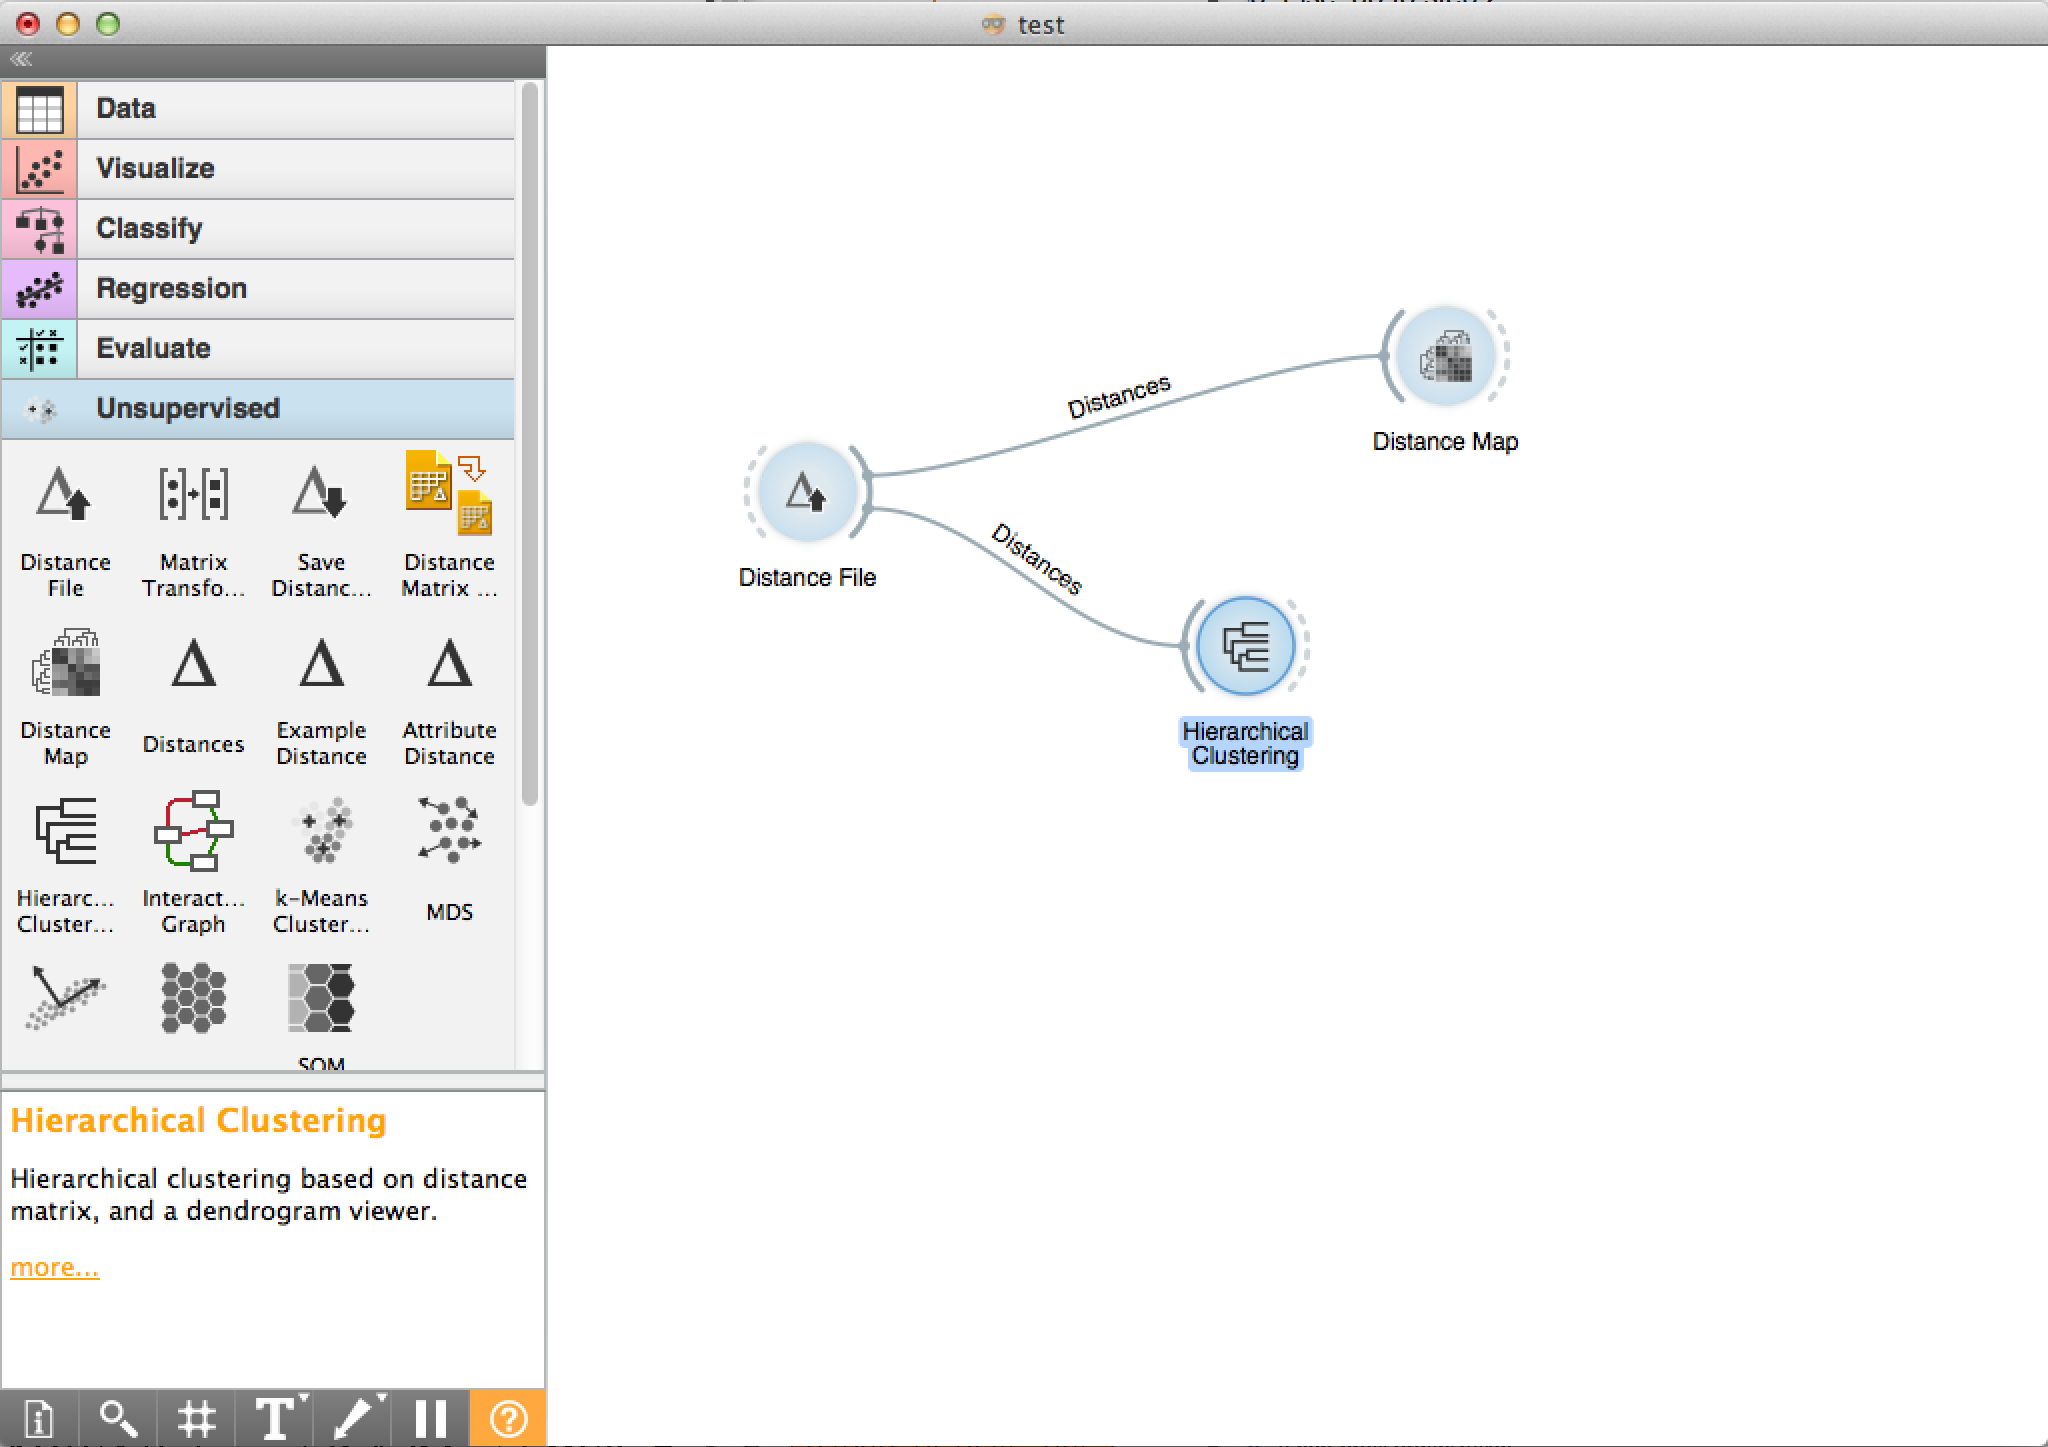
\includegraphics[width=\textwidth]{Figures/OrangeUI}
	\caption{The Orange widget-based User Interface}
	\label{fig:orangeUI}
\end{figure}
From here, the pair of clusters with the smallest
distance (or highest similarity) between the two is merged to form a new cluster.
The distance between this new cluster and the other clusters is updated to be
the max distance from the two merged clusters to the other clusters. This process
is repeated until a hierarchy of clusters has been formed and the data is merged
into one cluster. The Hierarchical Clustering widget displays this hierarchy
and allows the user to move the cutoff point, to increase the number/reduce the
size of clusters to their desired level.

\section{Conclusions}

We have found a large amount of research into the area of plagiarism detection
in source code, with little focus being on the similarity result itself. However
the algorithms presented do provide scope for creating a similarity analysis
project. Further, there are many applications already in production based around
the textual/token analysis ideas, and much less rigour has been applied to the
tree based approaches. This could be an interesting avenue to explore and is the
basis for our examination of the parse tree kernel algorithm. The Eclipse plugin
libraries provide an entry point to the java compiler and access to the parse
trees, and also has an API for the display of related information in the Eclipse
main window. The lack of modern, detailed data visualisation frameworks has led
us to look at external visualisation options, with Orange looking like a rich
framework with an easy to use UI that could be ideal for our needs.